\documentclass[12pt,a4paper,oneside,brazil]{abntex2}
\usepackage[utf8]{inputenc}
\usepackage[T1]{fontenc}
\usepackage[brazil]{babel}
\usepackage{graphicx}
\usepackage{lipsum} % Pacote para gerar texto fictício
\usepackage{helvet}
\usepackage{ragged2e}

\renewcommand{\familydefault}{\sfdefault}

\hypersetup{
    hidelinks
}

\titulo{Plataforma de Edição/Automação para trabalhos acadêmicos}
\autor{Higor Ferreira Alves Santos}
\orientador{Marcelo Antônio Adad}

\newcommand{\ies}{Pontifícia Universidade Católica de Goiás}
\newcommand{\escola}{Escola Politécnica e de Artes}
\newcommand{\curso}{Engenharia de Computação}

\newcommand{\grauOrientador}{Prof. M.E.E.}
\newcommand{\grauAluno}{Bacharel}
\newcommand{\bancaUm}{Miriam Gusmão}
\newcommand{\bancaDois}{}

\instituicao{%
    \ies
    \par
    \escola
    \par
    \curso
    }
\local{GOIÂNIA - GO}
\data{2023}

% Início do documento
\begin{document}

% Capa personalizada
\begin{capa}
    \center

    \OnehalfSpacing
    \ABNTEXchapterfont\bfseries{\textsc{\MakeUppercase{\imprimirinstituicao}}}

    \vfill

    % Incluir logotipo
    
\includegraphics[width=0.15\textwidth]{./src/assets/logo.png}

    \vfill

    \ABNTEXchapterfont\bfseries{\MakeUppercase{\imprimirtitulo}}

    \vfill

    \MakeUppercase{\imprimirautor}

    \vfill

    \bfseries{\MakeUppercase{\imprimirlocal}}

    \bfseries{\MakeUppercase{\imprimirdata}}
\end{capa}

% Folha de rosto personalizada
\begin{folhaderosto}

    \centering

    \MakeUppercase{\imprimirautor}

    \vfill

    \ABNTEXchapterfont\bfseries{\MakeUppercase{\imprimirtitulo}}

    \vfill

    \justifying
    \noindent\hspace*{70mm}%
    \begin{minipage}{\dimexpr\textwidth-70mm}
        \textnormal{
            Trabalho de Conclusão de Curso apresentado à
            \escola, da \ies, como parte dos
            requisitos para a obtenção do título de \grauAluno\,em
            \curso.\\\\
            Orientador:\\
            \begin{flushright}
                \grauOrientador \imprimirorientador
            \end{flushright}
            Banca examinadora:\\
            \begin{flushright}
                \bancaUm
                \bancaDois
            \end{flushright}
        }
    \end{minipage}

    \vfill

    \centering

    \bfseries{\imprimirlocal}

    \bfseries{\imprimirdata}
\end{folhaderosto}

% Folha de aprovação
\clearpage
    \centering
    \MakeUppercase{\imprimirautor}

    \vfill

    \ABNTEXchapterfont\bfseries{\MakeUppercase{\imprimirtitulo}}

    \vfill

    \justifying

    \textnormal{Trabalho de Conclusão de Curso aprovado em sua forma final pela Escola Politécnica e de
    Artes, da Pontifícia Universidade Católica de Goiás, para obtenção do título de \grauAluno\,em
    Engenharia de Computação, em: \_\_\_/ \_\_\_/ \_\_\_\_\_}

    \centering

    \vspace*{3cm}

    \begin{flushright}
    \rule{10cm}{0.4pt}\\
    \textnormal{Orientador: \grauOrientador \imprimirorientador}

    \vspace*{10mm}

    \rule{10cm}{0.4pt}\\
    \textnormal{Orientador1: \bancaUm}

    \vspace*{10mm}

    \rule{10cm}{0.4pt}\\
    \textnormal{Orientador2: \bancaDois}
    \end{flushright}

    \vspace*{6cm}

    \bfseries{\imprimirlocal}

    \bfseries{\imprimirdata}
\clearpage % Começa uma nova página para a folha de rosto

\pagenumbering{roman}

% Correção: Usar \tableofcontents para o Sumário
\tableofcontents
\clearpage
\listoffigures   % Lista de Figuras
\clearpage
\listoftables    % Lista de Tabelas
\clearpage

\pagenumbering{arabic}
\setcounter{page}{1}
\textual

\justifying
\normalfont

\chapter{Introdução}
Este é um exemplo de texto com uma nota de rodapé.\footnote{Aqui está o texto da nota de rodapé.} \lipsum[1]

\section{Subtítulo de Nível 1}
Texto com outra nota de rodapé.\footnote{Outro exemplo de nota de rodapé.} \lipsum[2-3]

\subsection{Subtítulo de Nível 2}
\lipsum[4]
\subsubsection{Subtítulo de Nível 3}
\lipsum[5]
\subsubsubsection{Subtítulo de Nível 4}
\lipsum[5]

\chapter{Revisão da Literatura}
\lipsum[6-7]

\chapter{Metodologia}
\lipsum[8-9]

\chapter{Resultados e Discussão}
\lipsum[10]

\begin{figure}[ht]
    \centering
    \caption{Exemplo de Figura}
    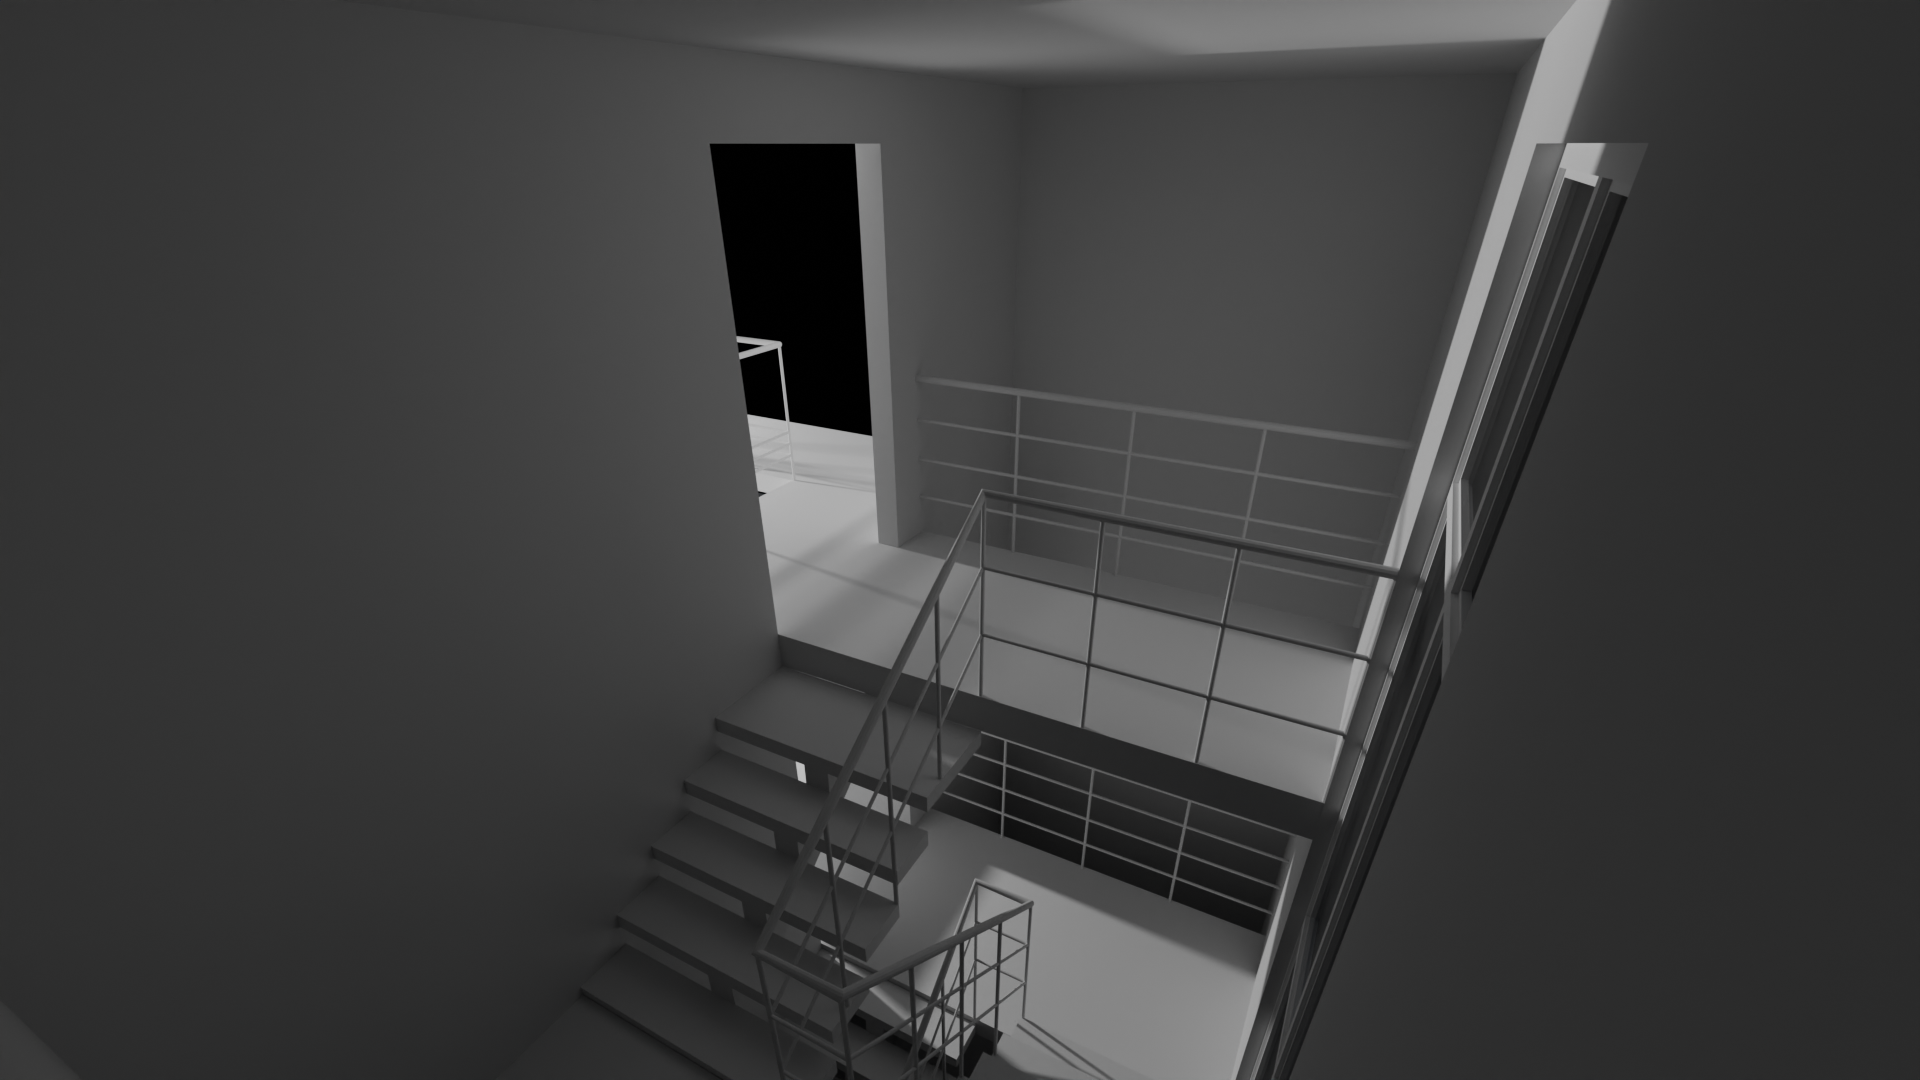
\includegraphics[width=1.0\textwidth]{./src/assets/untitled.png}
    \label{fig:exemplo}
    \textnormal{\fontsize{10pt}{12pt}Fonte: Autoria própria}
\end{figure}

\begin{table}[ht]
    \centering
    \caption{Exemplo de Tabela}
    \begin{tabular}{|c|c|c|}
        \hline
        Coluna 1 & Coluna 2 & Coluna 3 \\ \hline
        Item 1   & Item 2   & Item 3   \\ \hline
        Item 4   & Item 5   & Item 6   \\ \hline
    \end{tabular}
    \label{tab:exemplo}
    \\\textnormal{\fontsize{10pt}{12pt}Fonte: Autoria própria}
\end{table}

Lorem ipsum dolor sit amet consectetur, adipisicing elit. Veritatis expedita a distinctio. Culpa quidem dolores suscipit, aspernatur odit possimus voluptatem illo. Fugiat recusandae modi laboriosam qui ut commodi beatae velit?
Lorem ipsum dolor sit amet consectetur, adipisicing elit. Doloremque recusandae sint repudiandae fuga porro a, similique officiis quas eligendi tenetur ullam reiciendis officia cupiditate neque? Assumenda voluptatem soluta laudantium tempora inventore maiores possimus nam! Ut molestiae tempore quam dolore dolor assumenda. Accusamus, rem deserunt? Earum repellendus officia distinctio harum excepturi voluptatum deleniti rem, consequuntur sint illo voluptatibus quasi. Dolorum dolorem magnam obcaecati, autem consequuntur molestiae vero similique id. Suscipit eum consequuntur optio quisquam dolorum amet mollitia iure unde impedit labore cum dicta modi, voluptatum porro architecto molestiae ipsam maiores accusamus natus nihil? Iusto, dicta praesentium culpa molestias dignissimos nostrum qui excepturi nulla in! Reprehenderit animi, rerum beatae eius iste odio ea dignissimos, aut quaerat ratione voluptates dolorem architecto, autem recusandae!

Gostou? veja de novo a figura \ref{fig:exemplo}

\chapter{Conclusão}
\lipsum[11-12]

\bibliography{referencias}

\end{document}